\renewcommand{\thechapter}{\Roman{chapter}}
\chapter[]{LITERATURE REVIEW}
\renewcommand{\thechapter}{\arabic{chapter}}

\begingroup
\fontsize{12bp}{\baselineskip}\selectfont

\section{Data and Information}
	\subsection{Definitions}
		\begin{indentedblock}{4em}{0pt}
			Data refers to a collection of raw, unlabelled information which represents a set of truth/facts about the world \parencite{what_are_data_olson_karin}. Data comes in two main categories, quantitative and qualitative \parencite{what_are_data_lucina}. Quantitative data refers to data which has a distinct form, with unique categories and can be analyzed using objective numerical operations and methods, where qualitative data lacks a concrete structure and is highly context-dependent and subjective \parencite{quantitative_vs_qualitative_judith}. Quantitative data mostly consists of values that can be represented numerically (a person's height/weight, price of an object), while qualitative data refers to data about a subject such as nominal descriptions (a person's name, a novel's synopsis). This paper focuses on digital data, which is data represented as a sequence of symbols, mainly binary digits.
			
			\skiplines{1}
			
			The concept of data differs from information in that data serves as the foundation from which information is generated \parencite{what_are_data_lucina}. In essence, information is a specific interpretation of a given dataset, derived from their type and values, as well as their context and semantic meaning. In particular, the context in which a collection of data is acquired determines the set of valid interpretations of said data, which in turn affects the possible inferences i.e. potential information gathered from it \parencite{data_vs_information_mason}. Raw data in itself cannot be used directly, as it merely represents the attributes of a certain subject, without assigning to it any valid implication/insight. As such, the use of data involves converting it into information through analysis and contextualization \parencite{data_transformation_sanae_borrohou_et_al}.
			
			\skiplines{1}
			
			As the name suggests, information is the basis of all modern information technologies and systems such as search engines, recommendation systems, and artificial intelligence. These systems utilize information gathered from large datasets to gain knowledge, derive solutions and make decisions such as giving a custom-tailored recommendation to particular set of users in the case of recommendation systems, and generating responses in the case of AI. The amount of data generated daily has grown exponentially in the information age, with one estimate stating approximately 402.74 million terabytes are generated by electronic devices around the world daily, and an estimated 394 zettabytes will be generated by 2028 \parencite{data_growth_worldwide_taylor}. This prompts the need to develop a method for organizing, analyzing, and managing large batches of data efficiently and accurately. 
		\end{indentedblock}
	\subsection{Data classification}
		\begin{indentedblock}{4em}{0pt}
			Data classification is the process of assigning labels to data for better management purposes \parencites{data_classification_nist}{data_classification_sheela}. In short, data classification is the process of grouping data into different categories according to their characteristics for later processing and bookkeeping. Data classification allows for enhanced protection, security and risk management of data based on sensitivity and regulatory standards \parencites{role_of_data_classification_avery}{overview_of_data_classification_nguyen}{data_classification_nist}. Furthermore, data classification allows for better organization and retrieval of certain types of data, improving the accuracy and performance of information gathering. Data classification methods largely follows this specific sequence of steps: 1) defining classification criteria, 2) data discovery and sensitive data detection and 3) data labeling based on type, usage, and security requirements \parencite{data_classification_sheela}.
			
			\skiplines{1}
			
			Most forms of data, such as text, images, and video/audio recordings, are categorized as qualitative as they lack a formal, fixed set of attributes and structure. Furthermore, data with complex structures such as CAD files contain a large amount of features and attributes that form deep semantic relationships. As a result, these types of data cannot be easily classified using conventional methods as they rely on assumptions regarding the data's structure. Recent advancements in artificial intelligence systems such as natural language processing and deep learning have allowed for reliable, efficient classification of these datatypes \parencite{AI_driven_data_classification_moses}. In modern systems, vector embeddings have become the cornerstone that enables these capabilities, replacing the less efficient rule-based approach in natural language processing, and acting as the basis for deep learning systems such as convolutional/recurrent neural network models \parencites{text_representation_patil}{word_embedding_models_deepak}. This paper will focus on the use of vector embeddings as a method for enumerating and processing CAD files for classification purposes.
		\end{indentedblock}
	
\section{Vector Embeddings}
	\subsection{Definition and Purpose}
		\begin{indentedblock}{4em}{0pt}
%			\fontsize{12bp}{\baselineskip}\selectfont
			Vector embedding is defined as a method for converting and representing complex, unstructured data as a sequence of numerical values \parencites{vector_embeddings_pajo}{vector_embeddings_chitturi}. A vector embedding aims to create a compact, structured representation of an underlying datapoint while preserving the underlying context and semantic meanings contained in it \parencite{vector_embeddings_chitturi}. In other words, vector embeddings encode unstructured, context-rich data into points in an $n$-dimensional space, capturing the relationships of different data points in numeric form, allowing the data to be processed and analyzed using mathemathical operations \parencite{vector_embeddings_pajo}. This representation also renders the concept of ``distance'' as a quantifiable component in data analysis, where distance refers to semantic proximity/closeness in meaning \parencite{vector_database_sanjay}. In short, the distance between $n$-dimensional vector representation of two datapoints closely models the semantic relationship between the original data. 
			
			\skiplines{1}
			
			Vector embedding serves as a way to efficiently encode large datapoints such as texts, images, video and audio into a digestible, compact format that could be easily processed by other systems. Vector embeddings also allows data to be searched, indexed, and grouped using their semantic similarity \parencite{vector_database_taipalus}. One use case is in large language models, where models could be equipped with the ability to access external documents and data, allowing it to produce reliable output grounded on falsifiable truth \parencite{vector_embedding_omolayo}.
			
			\skiplines{1}
			
			Other similar methods for encoding qualitative, complex data have been developed, such as one-hot encoding, which encodes each datapoint as states represented as a sequence of $n$-bits, where all but one bit is set to `0', and the `1' bit represents the current state of the system \parencite{one_hot_encoding_samuels}. Another example is Bag of Words (BoW), which represents text as a ``bag''; an unordered, unstructured collection of its words, or keypoints in the case of an image \parencite{bag_of_words_qader}, and Term Frequency-Inverse Document Frequency (TF-IDF), which encodes words/keypoints as its number of occurrence and rarity inside a document \parencite{tf_idf_qaiser}. 
			
			\skiplines{1}
			
			Nonetheless, the methods listed previously face several limitations when compared to newer techniques such as vector embedding, such as the loss of semantic information such as the word order, grammatical structure, and other relevant context stored in the original. Other problems include the problem of dimensionality, which states that as the number of dimensions increase for a given set of data, the amount of available data becomes increasingly sparse and patterns more obscure \parencite{data_mining_robert}. This limitation also massively increases the compute power and memory required to store and process these encodings while also increasing the risk of errors \parencite{problem_of_dimensionality_trunk}. Vector embedding sidesteps these limitations by mapping similar items to vectors which have a close distance to each other, preserving semantic data and minimizing the number of features required. The shift from sparse, count-based encoding methods towards a more compact, learned encoding technique enables critical performance improvements in terms of data processing metrics such as compute time and output accuracy. 
			
		\end{indentedblock}
	\subsection{Embedding Models}
		\begin{indentedblock}{4em}{0pt}
			Although vector embedding offers several important advantages, such advantages require specialized, novel machine learning models that are capable of distilling complex relationships between datapoints into a compact dense vector representation while minimizing the amount of features/dimensions. These models capture context ingrained within datapoints by learning how to assign a connection between two neighboring words/parts of data \parencite[Chapter~4.1]{natural_language_processing_tran}. 
			
			\skiplines{1}
			
			Most embedding models could be categorized into two groups: static models that generate a single, fixed representation for a word/data segment, such as continuous BoW and Subword models \parencite{embedding_models_wang}, and contextual models such as Bidirectional Encoder Representations from Transformers (BERT) and its variants that generate unique representations of the same word depending on the current context \parencites{embedding_models_liu}{bert_devlin}. In recent times, contextual models have largely dominated due to their flexibility and better capabilities in terms of capturing the nuance and implicit interconnections between datapoints and its components. One popular example of this is the transformer architecture, which forms the basis the paper's research.
		\end{indentedblock}

\section{Transformer Architecture}
	\subsection{Architecture Overview}
		\begin{indentedblock}{4em}{0pt}
			Current state-of-the-art (SotA) embedding models are based on the transformer architecture, which acts as the foundation for commercial generative AI models such as ChatGPT, Gemini, and DeepSeek. Introduced in the seminal paper ``Attention Is All You Need''  \parencite{attention_is_all_you_need_vaswani}, instead of processing data sequentially, the architecture utilized a novel approach for sequential, recurrent processing tasks referred in the paper as \textbf{Self-Attention Mechanism}, replacing the recurrent, in-order structures of previous models like recurrent neural networks (RNNs) and long short-term memory models (LSTMs) \parencites{fundamentals_of_rnn_sherstinsky}{lstm_hochreiter}. This mechanism allows the model to process input sequences in parallel, which is critical for handling non-local graph structures present in STEP files. 
			
			\skiplines{1}			
			
			Central to this architecture is \textbf{Tokenization}, a process of dividing input data into smaller chunks referred to as tokens. The tokens are represented as numeric vectors, reducing the amount of storage and compute needed for further processing. The literature dictates two main paradigms of tokenizing input data, full word and subword tokenization. Full word tokenization, as it implies, splits input data based on a pre-defined separator, such as whitespace in text. The above method have largely been replaced by its counterpart, which divides input data into smaller subparts that has no fixed separator. Examples of subword tokenization include Byte-Pair Encoding (BPE) and WordPiece \parencites{subword_tokenization_method_burak}{bpe_kozma}{bert_devlin}. The tokens generated from the process are then used as the main input data of the self-attention mechanism. While traditional models utilize subword tokenizers like BPE to parse natural language, this research adapts the concept to the geometric domain. Just as an LLM tokenizes words to understand a sentence, the proposed architecture tokenizes topological entities (e.g., surfaces, curves) to "read" a 3D object. These geometric tokens are then processed by the attention mechanism to generate semantic descriptions.
			
			\skiplines{1}
			
			The self-attention mechanism detailed in the transformer architecture improves upon previous systems by enabling models to evaluate the importance of the surrounding parts of an input sequence, regardless of its ordering. For instance, consider the sentence ``The dog barked at the cat to drive it away.'' Using self-attention, transformer-based models can correctly associate the word ``it'' with the word ``cat'' rather than ``dog'' \parencite{attention_is_all_you_need_vaswani}. This capability of handling remote dependencies and understand context allows it to outperform previous architectures. The details of the mechanism lies in the novel components that make up the architecture, forming a deep network. In particular, the transformer model's functionality and reliability is the outcome from combining two key components, encoders and decoders. \autoref{fig:encoder-decoder} details the architecture of a standard transformer.
			
			\begin{figure}[H]
				\centering
				\includegraphics[width=0.5\linewidth]{"../Images/ENCODER DECODER"}
				\caption{Standard Transformer Architecture consisting of an Encoder and Decoder \parencite{attention_is_all_you_need_vaswani}}
				\label{fig:encoder-decoder}
			\end{figure}
			
		\end{indentedblock} 
	\subsection{Encoder-Decoder}
		\begin{indentedblock}{4em}{0pt}
			The encoder-decoder components consists of several blocks/subcomponents that in turn form the basis of a transformer layer, which are then stacked continuously to build the complex models. The encoder functions as a processing layer for the entire input sequence, aiming to build a rich, contextualized numerical representation utilizing the self-attention mechanism. The encoder is implemented as two main parts:
			\begin{enumerate}
				\item {
					\textbf{Multi-Head Self-Attention:} \\
					The self-attention of the transformer is employed as different units/heads working in parallel, allowing the model to learn different types of relationships from the input data simultaneously \parencite{multi_head_self_attention_voita}. Each ``head'' is tasked with learning a different aspect of the given sequence. For instance, one head might focus on syntactic relationships while another learns semantic ones. This functionality is done through projecting the input data into different representation subspaces and applying self-attention in parallel. The final result is a vector generated by applying a linear transform to the concatenation of the heads' output \parencite{attention_is_all_you_need_vaswani}
				}
				\item {
					\textbf{Position-wise Feed-Forward Networks (FFN):} \\
					The next step consists of passing the token vectors gathered and weighted from the attention mechanism through a feed-forward neural network. The subcomponent consists of two linear neural network layer with a non-linear activation function in between, such as ReLU. It enriches each token's representation by first expanding the vector's dimension (i.e. 512 to 2048), applying an activation layer and resizing the vectors back into its original size. This process allows the model to extract deep, interconnected patterns hidden within the data. Furthermore, the network acts as a key-value store for patterns learned during training, and its output represents a distribution of tokens containing said patterns \parencite{ffn_geva}.
				}
			\end{enumerate}
			
			The parallel nature of self-attention makes it difficult to retain information regarding sequence ordering. Hence, positional encodings in the form of special vectors are added to the embedddings to mitigate this limitation. The positional encoding vectors are generated using sinusoidal functions with different frequencies that represent positions of tokens inside the sequence \parencite{attention_is_all_you_need_vaswani}. After the encoding process, the result generated by the encoder is passed through a decoder that remaps the resulting vectors back into tokens that forms the final output sequence. The decoder achieves this through three steps:
			
			\begin{enumerate}
				\item {
					\textbf{Masked Multi-Head Self-Attention:}\\
					The first step of the decoding sequence is similar with encoding, with a key difference being he lack of a lookahead for future tokens. This is done to prevent model overfitting as knowing future tokens might embed irrelevant connections into the model.
				}
				\item {
					\textbf{Cross-attention:} \\
					Another change made in the decoding process is the addition of a cross-attention layer. The layer acts as a critical link between the encoder and decoder that functions as a window for the decoder to look at the encoder's final output. The encoder uses its internal state as a query in the form of a vector and relates it to the vector set generated by the encoder. This process enabels the decoder to determine the most relevant parts of the input and its relation to the final output \parencite{attention_is_all_you_need_vaswani}.
				}
				\item {
					\textbf{Position-wise Feed-Forward Networks (FFN):} \\
					The final decoding step is similar to the encoding process with no changes.
				}
			\end{enumerate}
			
			Enabling effective training of densely-layered networks require proper integration of the encoder and decoder. These requirements prompts the use of two operations which are applied post-encoding and decoding to ensure stability and effective training. The integration involves adding a residual connection layer that adds the original input vector with the output to minimize the vanishing gradient problem. Next, the vectors are normalized and stabilized, ensuring a smoother and reliable training process. The architectural decisions that make up the model allows the connections between each token to be filtered and strengthened based on the input's context, and allows the model to retain more information from its training data \parencite{attention_is_all_you_need_vaswani}.
		\end{indentedblock}
\section{Related Works}
	\begin{indentedblock}{4em}{0pt}
		Early attempts at classifying CAD files mainly used feature descriptors such as Zernike and Reeb graph descriptors to determine the category of a CAD model based on shape and function \parencite{cad_ip}.  Several other works focuses on 2D based methods such as utilizing machine learning to classify over 1600 CAD files using random forest, support vector and fully-connected neural network models by identifying 45 different basic shapes \parencite{ml_machalica}, with subsequent approaches combining GNN to measure and group CAD files based on their similarities in geometry \parencite{cad_classification_roj}. More examples of this type include RotationNet, which utilizes images  of the same 3D objects from different angles to estimate its pose and category \parencite{rotationnet_kanezaki}. 
		
		\skiplines{1}
		
		Different category of related studies uses a 3D-based approach, with one leveraging the use of 3D grid representation (voxels) of the CAD file and applying a 3-dimensional-CNN that could detect and categorize features \parencite{voxnet_maturana}, and another applies a Mask-recurrent CNN model to extract 3D objects from a single 2D RGB image which can then be classified \parencite{can_mrcnn}. Works such as PointNet utilizes 3D point clouds to estimate the class of an object \parencite{pointnet_qi}. A different classification uses a custom 3D representation named PANORAMA and feeding the result to a CNN to find keypoints and classify the CAD based on the detected features \parencites{panorama_papadakis}{panorama_cnn_retrieval_sfikas}{panorama_cnn_ensemble_sfikas}. Newer 3D-based approaches utilizes graph-based techniques to make use of the graph-like structure of CAD files such as STEP, with one work using Graph-based Neural Network (GNN) to categorize certain CAD STEP files into 7 different classes \parencite{gnn_mandelli}. However, a research gap in previous works can be identified, since the cited works are limited to classifying a fixed class of CAD objects, such as bolts, and cannot be used to create a general description of objects not specified in the class dataset. 
		
		\skiplines{1}
		
		Another method applies a Feature Directed Acyclic Graph (FDAG) to determine the dependency between the shapes of CAD models which are then optimized until only the fundamental features and shapes remain. The shapes can then be compared to CAD models to determine their resemblance to the shapes used as a query \parencite{cnn_li}. One graph based method also utilizes the structure of STEP files to generate an attribute graph which can then be used as a measure for shape similarity \parencites{cad_el_mehalawi}{indexing_el_mehalawi}. However, while these graph-theoretic approaches excel at topological retrieval, they remain disconnected from the semantic intent of the design. 
		
		\skiplines{1}
		
		To bridge the gap between geometric topology and natural language, recent frameworks have turned to multi-modal learning. Text2CAD provides a seminal contribution by pairing natural language with CAD geometry, its methodology relies entirely on Programmatic Synthesis \parencite{text2cad_khan}. The dataset is constructed by first generating CAD scripts and then using Large Language Models (LLMs) to reverse-engineer textual descriptions from the code. Nevertheless, the approach introduces a research gap as real-world industry STEP files (ISO 10303-21) rarely contain the clean construction history (e.g., Extrude, Revolve) found in Text2CAD. \autoref{fig:text2cad} details the overall flow of Text2CAD. They are often fixed Boundary Representations (B-Reps) containing only explicit surfaces and topology. Therefore, a model trained solely on Text2CAD fails to interpret the vast majority of preexisting CAD files. Moreover, the research focuses on generating the step-by-step geometric operations required for reconstruction (e.g. "Extrude by 2cm"). While this results in precise parametric descriptions, the model effectively describes the object's recipe without understanding what the object is. For instance, while it may generate highly accurate construction steps for a set of interlocking toothed cylinders and shafts by specifying exact relative measurements for every extrude and cut, it frequently fails to recognize or categorize the resulting assembly by its fundamental functional identity: a Gearbox. Consequently, the model provides the fabrication steps but lacks the capability to semantically categorize said object.
		
		\skiplines{1}
		
		To overcome the dependency on synthetic construction history and the lack of functional understanding, this study introduces a tokenizer and annotation pipeline designed explicitly for Reconstruction-Free B-Rep Graphs. Furthermore, to ensure the model captures the high-level semantic identity of components rather than just their geometric recipe, this research employs a Human-in-the-Loop (HITL) protocol to directly author and verify the dataset. This verification process guarantees that the descriptions align with the visual reality of the part, prioritizing functional categorization over procedural fabrication.
		
		\begin{figure}[H]
			\centering
			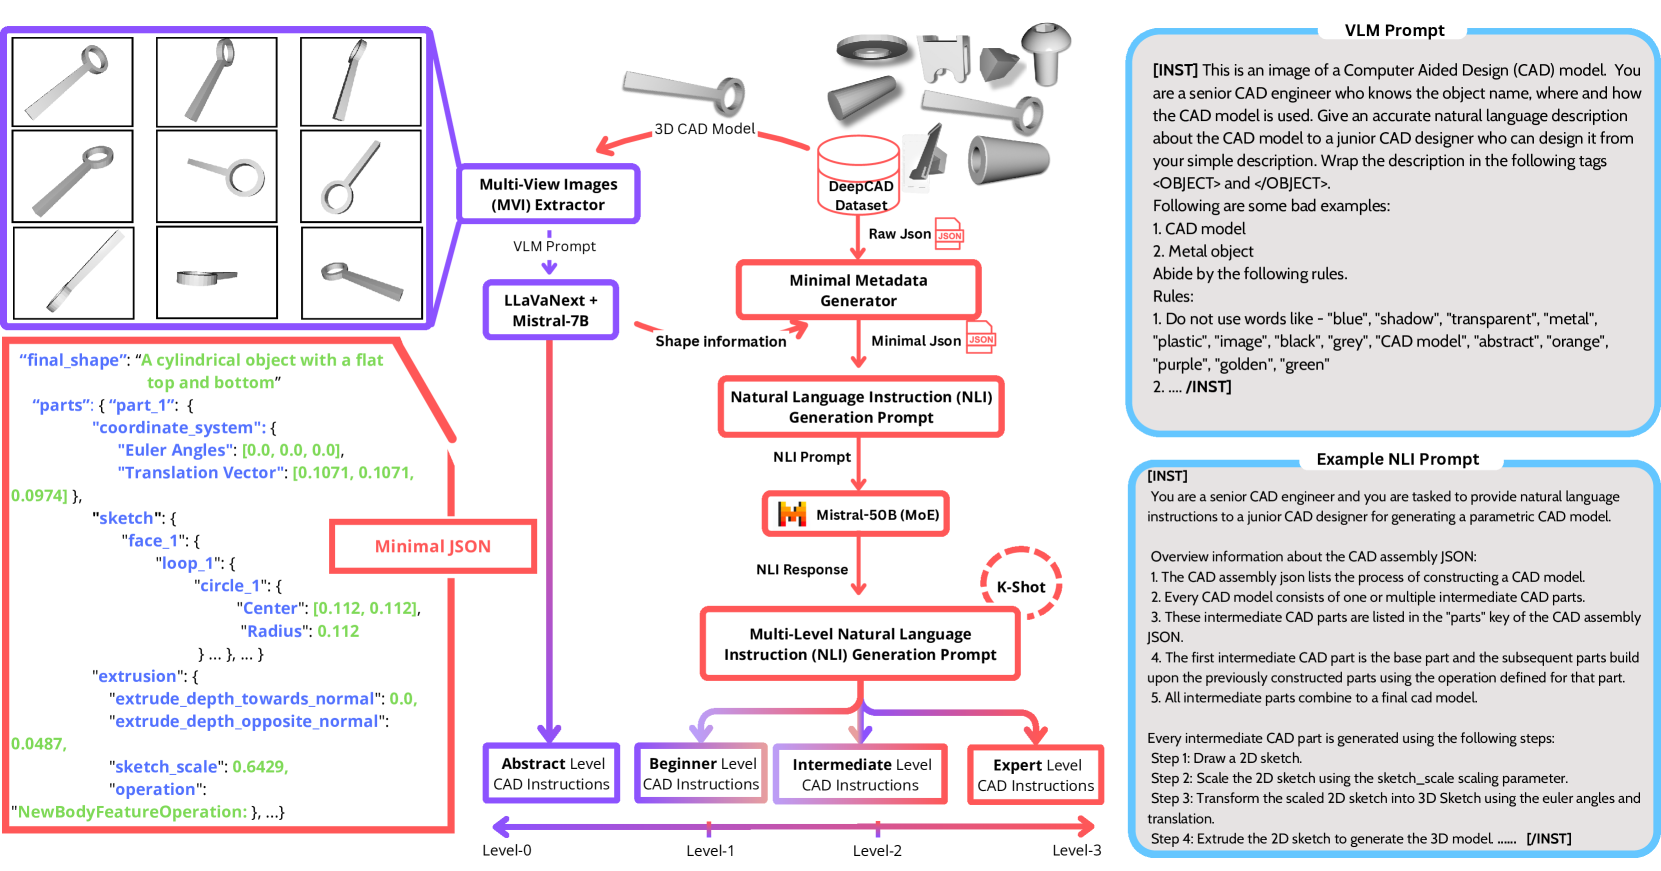
\includegraphics[width=1.25\linewidth, pagecenter]{../Images/Text2CAD}
			\caption{Text2CAD Annotation Generation Pipeline \parencite{text2cad_khan}}
			\label{fig:text2cad}
		\end{figure}
		
	\end{indentedblock}

\endgroup
